%!TEX TS-program = xelatex
\documentclass[10pt,oneside]{article}
\usepackage[fontsize=9pt]{scrextend}

\usepackage[english]{babel}

\usepackage{amsmath,amssymb,amsfonts}
\usepackage[utf8]{inputenc}
\usepackage[T1]{fontenc}
\usepackage{stix2}
\usepackage[scaled]{helvet}
\usepackage[scaled]{inconsolata}

\usepackage{lastpage}

\usepackage{setspace}

\usepackage{ccicons}

\usepackage[hang,flushmargin]{footmisc}

\usepackage{geometry}

\setlength{\parindent}{0pt}
\setlength{\parskip}{6pt plus 2pt minus 1pt}

\usepackage{fancyhdr}
\renewcommand{\headrulewidth}{0pt}\providecommand{\tightlist}{%
  \setlength{\itemsep}{0pt}\setlength{\parskip}{0pt}}

\makeatletter
\newcounter{tableno}
\newenvironment{tablenos:no-prefix-table-caption}{
  \caption@ifcompatibility{}{
    \let\oldthetable\thetable
    \let\oldtheHtable\theHtable
    \renewcommand{\thetable}{tableno:\thetableno}
    \renewcommand{\theHtable}{tableno:\thetableno}
    \stepcounter{tableno}
    \captionsetup{labelformat=empty}
  }
}{
  \caption@ifcompatibility{}{
    \captionsetup{labelformat=default}
    \let\thetable\oldthetable
    \let\theHtable\oldtheHtable
    \addtocounter{table}{-1}
  }
}
\makeatother

\usepackage{array}
\newcommand{\PreserveBackslash}[1]{\let\temp=\\#1\let\\=\temp}
\let\PBS=\PreserveBackslash

\usepackage[breaklinks=true]{hyperref}
\hypersetup{colorlinks,%
citecolor=blue,%
filecolor=blue,%
linkcolor=blue,%
urlcolor=blue}
\usepackage{url}

\usepackage{caption}
\setcounter{secnumdepth}{0}
\usepackage{cleveref}

\usepackage{graphicx}
\makeatletter
\def\maxwidth{\ifdim\Gin@nat@width>\linewidth\linewidth
\else\Gin@nat@width\fi}
\makeatother
\let\Oldincludegraphics\includegraphics
\renewcommand{\includegraphics}[1]{\Oldincludegraphics[width=\maxwidth]{#1}}

\usepackage{longtable}
\usepackage{booktabs}

\usepackage{color}
\usepackage{fancyvrb}
\newcommand{\VerbBar}{|}
\newcommand{\VERB}{\Verb[commandchars=\\\{\}]}
\DefineVerbatimEnvironment{Highlighting}{Verbatim}{commandchars=\\\{\}}
% Add ',fontsize=\small' for more characters per line
\usepackage{framed}
\definecolor{shadecolor}{RGB}{248,248,248}
\newenvironment{Shaded}{\begin{snugshade}}{\end{snugshade}}
\newcommand{\KeywordTok}[1]{\textcolor[rgb]{0.13,0.29,0.53}{\textbf{#1}}}
\newcommand{\DataTypeTok}[1]{\textcolor[rgb]{0.13,0.29,0.53}{#1}}
\newcommand{\DecValTok}[1]{\textcolor[rgb]{0.00,0.00,0.81}{#1}}
\newcommand{\BaseNTok}[1]{\textcolor[rgb]{0.00,0.00,0.81}{#1}}
\newcommand{\FloatTok}[1]{\textcolor[rgb]{0.00,0.00,0.81}{#1}}
\newcommand{\ConstantTok}[1]{\textcolor[rgb]{0.00,0.00,0.00}{#1}}
\newcommand{\CharTok}[1]{\textcolor[rgb]{0.31,0.60,0.02}{#1}}
\newcommand{\SpecialCharTok}[1]{\textcolor[rgb]{0.00,0.00,0.00}{#1}}
\newcommand{\StringTok}[1]{\textcolor[rgb]{0.31,0.60,0.02}{#1}}
\newcommand{\VerbatimStringTok}[1]{\textcolor[rgb]{0.31,0.60,0.02}{#1}}
\newcommand{\SpecialStringTok}[1]{\textcolor[rgb]{0.31,0.60,0.02}{#1}}
\newcommand{\ImportTok}[1]{#1}
\newcommand{\CommentTok}[1]{\textcolor[rgb]{0.56,0.35,0.01}{\textit{#1}}}
\newcommand{\DocumentationTok}[1]{\textcolor[rgb]{0.56,0.35,0.01}{\textbf{\textit{#1}}}}
\newcommand{\AnnotationTok}[1]{\textcolor[rgb]{0.56,0.35,0.01}{\textbf{\textit{#1}}}}
\newcommand{\CommentVarTok}[1]{\textcolor[rgb]{0.56,0.35,0.01}{\textbf{\textit{#1}}}}
\newcommand{\OtherTok}[1]{\textcolor[rgb]{0.56,0.35,0.01}{#1}}
\newcommand{\FunctionTok}[1]{\textcolor[rgb]{0.00,0.00,0.00}{#1}}
\newcommand{\VariableTok}[1]{\textcolor[rgb]{0.00,0.00,0.00}{#1}}
\newcommand{\ControlFlowTok}[1]{\textcolor[rgb]{0.13,0.29,0.53}{\textbf{#1}}}
\newcommand{\OperatorTok}[1]{\textcolor[rgb]{0.81,0.36,0.00}{\textbf{#1}}}
\newcommand{\BuiltInTok}[1]{#1}
\newcommand{\ExtensionTok}[1]{#1}
\newcommand{\PreprocessorTok}[1]{\textcolor[rgb]{0.56,0.35,0.01}{\textit{#1}}}
\newcommand{\AttributeTok}[1]{\textcolor[rgb]{0.77,0.63,0.00}{#1}}
\newcommand{\RegionMarkerTok}[1]{#1}
\newcommand{\InformationTok}[1]{\textcolor[rgb]{0.56,0.35,0.01}{\textbf{\textit{#1}}}}
\newcommand{\WarningTok}[1]{\textcolor[rgb]{0.56,0.35,0.01}{\textbf{\textit{#1}}}}
\newcommand{\AlertTok}[1]{\textcolor[rgb]{0.94,0.16,0.16}{#1}}
\newcommand{\ErrorTok}[1]{\textcolor[rgb]{0.64,0.00,0.00}{\textbf{#1}}}
\newcommand{\NormalTok}[1]{#1}

\newlength{\cslhangindent}
\setlength{\cslhangindent}{1.5em}
\newlength{\csllabelwidth}
\setlength{\csllabelwidth}{3em}
\newenvironment{CSLReferences}[3] % #1 hanging-ident, #2 entry spacing
 {% don't indent paragraphs
  \setlength{\parindent}{0pt}
  % turn on hanging indent if param 1 is 1
  \ifodd #1 \everypar{\setlength{\hangindent}{\cslhangindent}}\ignorespaces\fi
  % set entry spacing
  \ifnum #2 > 0
  \setlength{\parskip}{#2\baselineskip}
  \fi
 }%
 {}
\usepackage{calc} % for \widthof, \maxof
\newcommand{\CSLBlock}[1]{#1\hfill\break}
\newcommand{\CSLLeftMargin}[1]{\parbox[t]{\maxof{\widthof{#1}}{\csllabelwidth}}{#1}}
\newcommand{\CSLRightInline}[1]{\parbox[t]{\linewidth}{#1}}
\newcommand{\CSLIndent}[1]{\hspace{\cslhangindent}#1}\usepackage[table,dvipsnames]{xcolor}

\geometry{includemp,
            letterpaper,
            top=2.4cm,
            bottom=2.4cm,
            left=1.0cm,
            right=1.0cm,
            marginparwidth=5cm,
            marginparsep=1.0cm}

\usepackage[singlelinecheck=off]{caption}

\captionsetup{
  font={small},
  labelfont={bf},
  format=plain,
  labelsep=quad
}

\usepackage{floatrow}

\floatsetup[figure]{margins=hangright,
              facing=no,
              capposition=beside,
              capbesideposition={center,outside},
              floatwidth=\textwidth}

% \floatsetup[table]{margins=hangright,
%              facing=no,
%              capposition=beside,
%              capbesideposition={center,outside},
%              floatwidth=\textwidth}

\pagestyle{plain}

\setcounter{secnumdepth}{5}

\usepackage{titlesec}

\titleformat{\section}[block]
{\normalfont\large\sffamily}
{\thesection}{.5em}{\titlerule\\[.8ex]\bfseries}

\titleformat{\subsection}[runin]
{\normalfont\fontseries{b}\selectfont\filright\sffamily}
{\thesubsection.}{.5em}{}

\titleformat{\subsubsection}[runin]
{\normalfont\itshape\rmfamily\bfseries}{\thesubsubsection}{1em}{}

\fancypagestyle{firstpage}
{
   \fancyhf{}
   \renewcommand{\headrulewidth}{0pt}
   \fancyfoot[R]{\footnotesize\ccby}
   \fancyfoot[L]{\footnotesize\sffamily\today}
}

\fancypagestyle{normal}
{
  \fancyhf{}
  \fancyfoot[R]{\footnotesize\sffamily\thepage\ of \pageref*{LastPage}}
}

\usepackage{tikz}
\begin{document}
\pagestyle{normal}
\thispagestyle{firstpage}

\newcommand{\colorRule}[3][black]{\textcolor[HTML]{#1}{\rule{#2}{#3}}}

\noindent {\LARGE \textbf{\textsf{Building a better metaweb: predicting
spatially and temporally explicit alpine plant-pollinator interaction
networks}}}

\medskip
\begin{flushleft}
{\small
%
\href{https://orcid.org/0000-0002-6506-6487}{Michael D.\,Catchen}%
%
\,\textsuperscript{1,2}, %
Paul\,CaraDonna%
%
\,\textsuperscript{3,4}, %
Jane E.\,Ogilvie%
%
\,\textsuperscript{3}, %
\href{https://orcid.org/0000-0001-9051-0597}{Francis\,Banville}%
%
\,\textsuperscript{3}, %
\href{https://orcid.org/0000-0002-2151-6693}{Dominique\,Caron}%
%
\,\textsuperscript{1,2}, %
\href{https://orcid.org/0000-0002-6248-3007}{Philippe\,Desjardins-Proulx}%
%
\,\textsuperscript{5,2}, %
\href{https://orcid.org/0000-0001-9019-0108}{Norma R.\,Forero-Muñoz}%
%
\,\textsuperscript{5,2}, %
\href{https://orcid.org/0000-0002-4498-7076}{Dominique\,Gravel}%
%
\,\textsuperscript{6,2}, %
\href{https://orcid.org/0000-0002-6004-4027}{Laura\,Pollock}%
%
\,\textsuperscript{1,2}, %
\href{https://orcid.org/0000-0001-6067-1349}{Tanya\,Strydom}%
%
\,\textsuperscript{5,2}, %
\href{https://orcid.org/0000-0002-0735-5184}{Timothée\,Poisot}%
%
\,\textsuperscript{5,2}, %
Julian\,Resasco%
%
\,\textsuperscript{7}, %
\href{https://orcid.org/0000-0001-6075-8081}{Andrew\,Gonzalez}%
%
\,\textsuperscript{1,2}
\vskip 1em
\textsuperscript{1}\,McGill University; \textsuperscript{2}\,Québec
Centre for Biodiversity Sciences; \textsuperscript{3}\,Rocky Mountain
Biological Laboratory; \textsuperscript{4}\,Chicago Bontanic
Garden; \textsuperscript{5}\,Université de
Montréal; \textsuperscript{6}\,Université de
Sherbrooke; \textsuperscript{7}\,University of Colorado Boulder\\
\vskip 1em
\textbf{Correspondance to:}\\
Michael D. Catchen --- \texttt{michael.catchen@mail.mcgill.ca}\\
}
\end{flushleft}

\vskip 2em
\makebox[0pt][l]{\colorRule[CCCCCC]{2.0\textwidth}{0.5pt}}
\vskip 2em
\noindent

\marginpar{\vskip 1em\flushright
{\small{\bfseries Keywords}:\par
species interactions\\ecological
forecasting\\pollinators\\bumbleebees\\network ecology\\}
}




        {\bfseries Purpose:}\,This template provides a series of scripts
to render a markdown document into an interactive website and a series
of PDFs.\\%
        {\bfseries Motivation:}\,It makes collaborating on text with
GitHub easier, and means that we never need to think about the
output.\\%
        {\bfseries Internals:}\,GitHub actions and a series of python
scritpts. The markdown is handled with \texttt{pandoc}.\\%
    

\vskip 2em
\makebox[0pt][l]{\colorRule[CCCCCC]{2.0\textwidth}{0.5pt}}
\vskip 2em

\hypertarget{abstract}{%
\subsection{Abstract}\label{abstract}}

Using a data set of {[}DESCRIBE EACH DATASET IN A NICE WAY{]}, we
predict a spatiotemporally explicit metaweb of interactions between
bumblebees (\emph{Bombus}) and wildflowers (within \emph{find clade}).
We integrate this data with crowdsourced occurrence data and climate
data to {[}best paint the picture of the Colorado bumblebee-plant
metaweb{]}. Using temporal climate data, we forecast how the
spatiotemporal overlap of interacting species will change under proposed
climate scenarios. We use this to estimate what interactions between
bees and plants need the most attention to prevent the spatiotemporal
decoupling of an interactions from threatening ecosystem functioning or
the persistence of a species.

\hypertarget{introduction}{%
\section{Introduction}\label{introduction}}

Species interactions are important. It is ultimately interactions
between individuals of different species that drive the structure,
dynamics, and persistence of ecosystems, and the abundance and diversity
of the species within them. Plant-pollinator interactions specifically
drive the function and persistence of ``architecture of biodiversity''
(Bascompte \& Jordano 2007). However, we are far from a robust
understanding of plant-pollinator networks. This is because sampling
interactions is costly. Interactions vary in space and time (Poisot
\emph{et al.} 2015)---particularlly relevent in this system {[}Paul
phenology cite{]}. This is why there is interest in using models to
predict interactions from sparse data (\textbf{Strydom2021?}). In this
paper, we combine several datasets, each spanning several years, to
produce spatially and temporally explicit predictions of the bumblebee
(genus \emph{Bombus}) and wildflower pollination network across the
state of Colorado.

We do this in two parts: (1) metaweb prediction and (2) conditioning our
metaweb prediction on co-occurrence probability. First, we build a model
to predict the metaweb---the network of \emph{all} interactions,
aggregated across all times and spatial locations---of \emph{Bombus} and
wildflower species across Colorado. (Why do this? The metaweb is more
predictable than local interactions.) We do this using network embedding
(\textbf{cite?}). Network embedding takes each node in the network
(either a bumblebee or a wildflower) and represents it in a latent \(n\)
dimensional space. Combination of running models on Temporal niche (T),
Phylogenetic niche (P), Environmental niche (E), and relative abundance
in community (RA).

Second, we then use this metaweb to predict the structure of networks at
specific locations and times of year (Gravel \emph{et al.} 2019).
Finally we suggest a map of sampling priority, which suggests the
locations to sample that will best improve our understanding of the
Colorado \emph{Bombus} pollination metaweb.

Why is this good for science, what does this contribute to our
understanding of plant-pollinator ints, networks, Bombus, predictive
models, etc., and how can these results be useful.

\hypertarget{data}{%
\section{Data}\label{data}}

We use three separate field datasets to estimate the Colorado
\emph{Bombus} metaweb.

\hypertarget{methods}{%
\section{Methods}\label{methods}}

\textbf{\emph{Concept Fig}}

\hypertarget{metaweb-model}{%
\section{Metaweb Model}\label{metaweb-model}}

\hypertarget{phylogeny-construction}{%
\subsection{Phylogeny Construction}\label{phylogeny-construction}}

\hypertarget{feature-embedding}{%
\subsection{Feature Embedding}\label{feature-embedding}}

\hypertarget{relative-abundance}{%
\subsubsection{Relative Abundance}\label{relative-abundance}}

\hypertarget{phylogenetic-features}{%
\subsubsection{Phylogenetic features}\label{phylogenetic-features}}

\hypertarget{environmental-niche-features}{%
\subsubsection{Environmental niche
features}\label{environmental-niche-features}}

\hypertarget{temporal-niche-features}{%
\subsubsection{Temporal niche features}\label{temporal-niche-features}}

\hypertarget{metaweb-model-fitting-and-validation}{%
\subsection{Metaweb Model Fitting and
Validation}\label{metaweb-model-fitting-and-validation}}

\begin{figure}
\centering
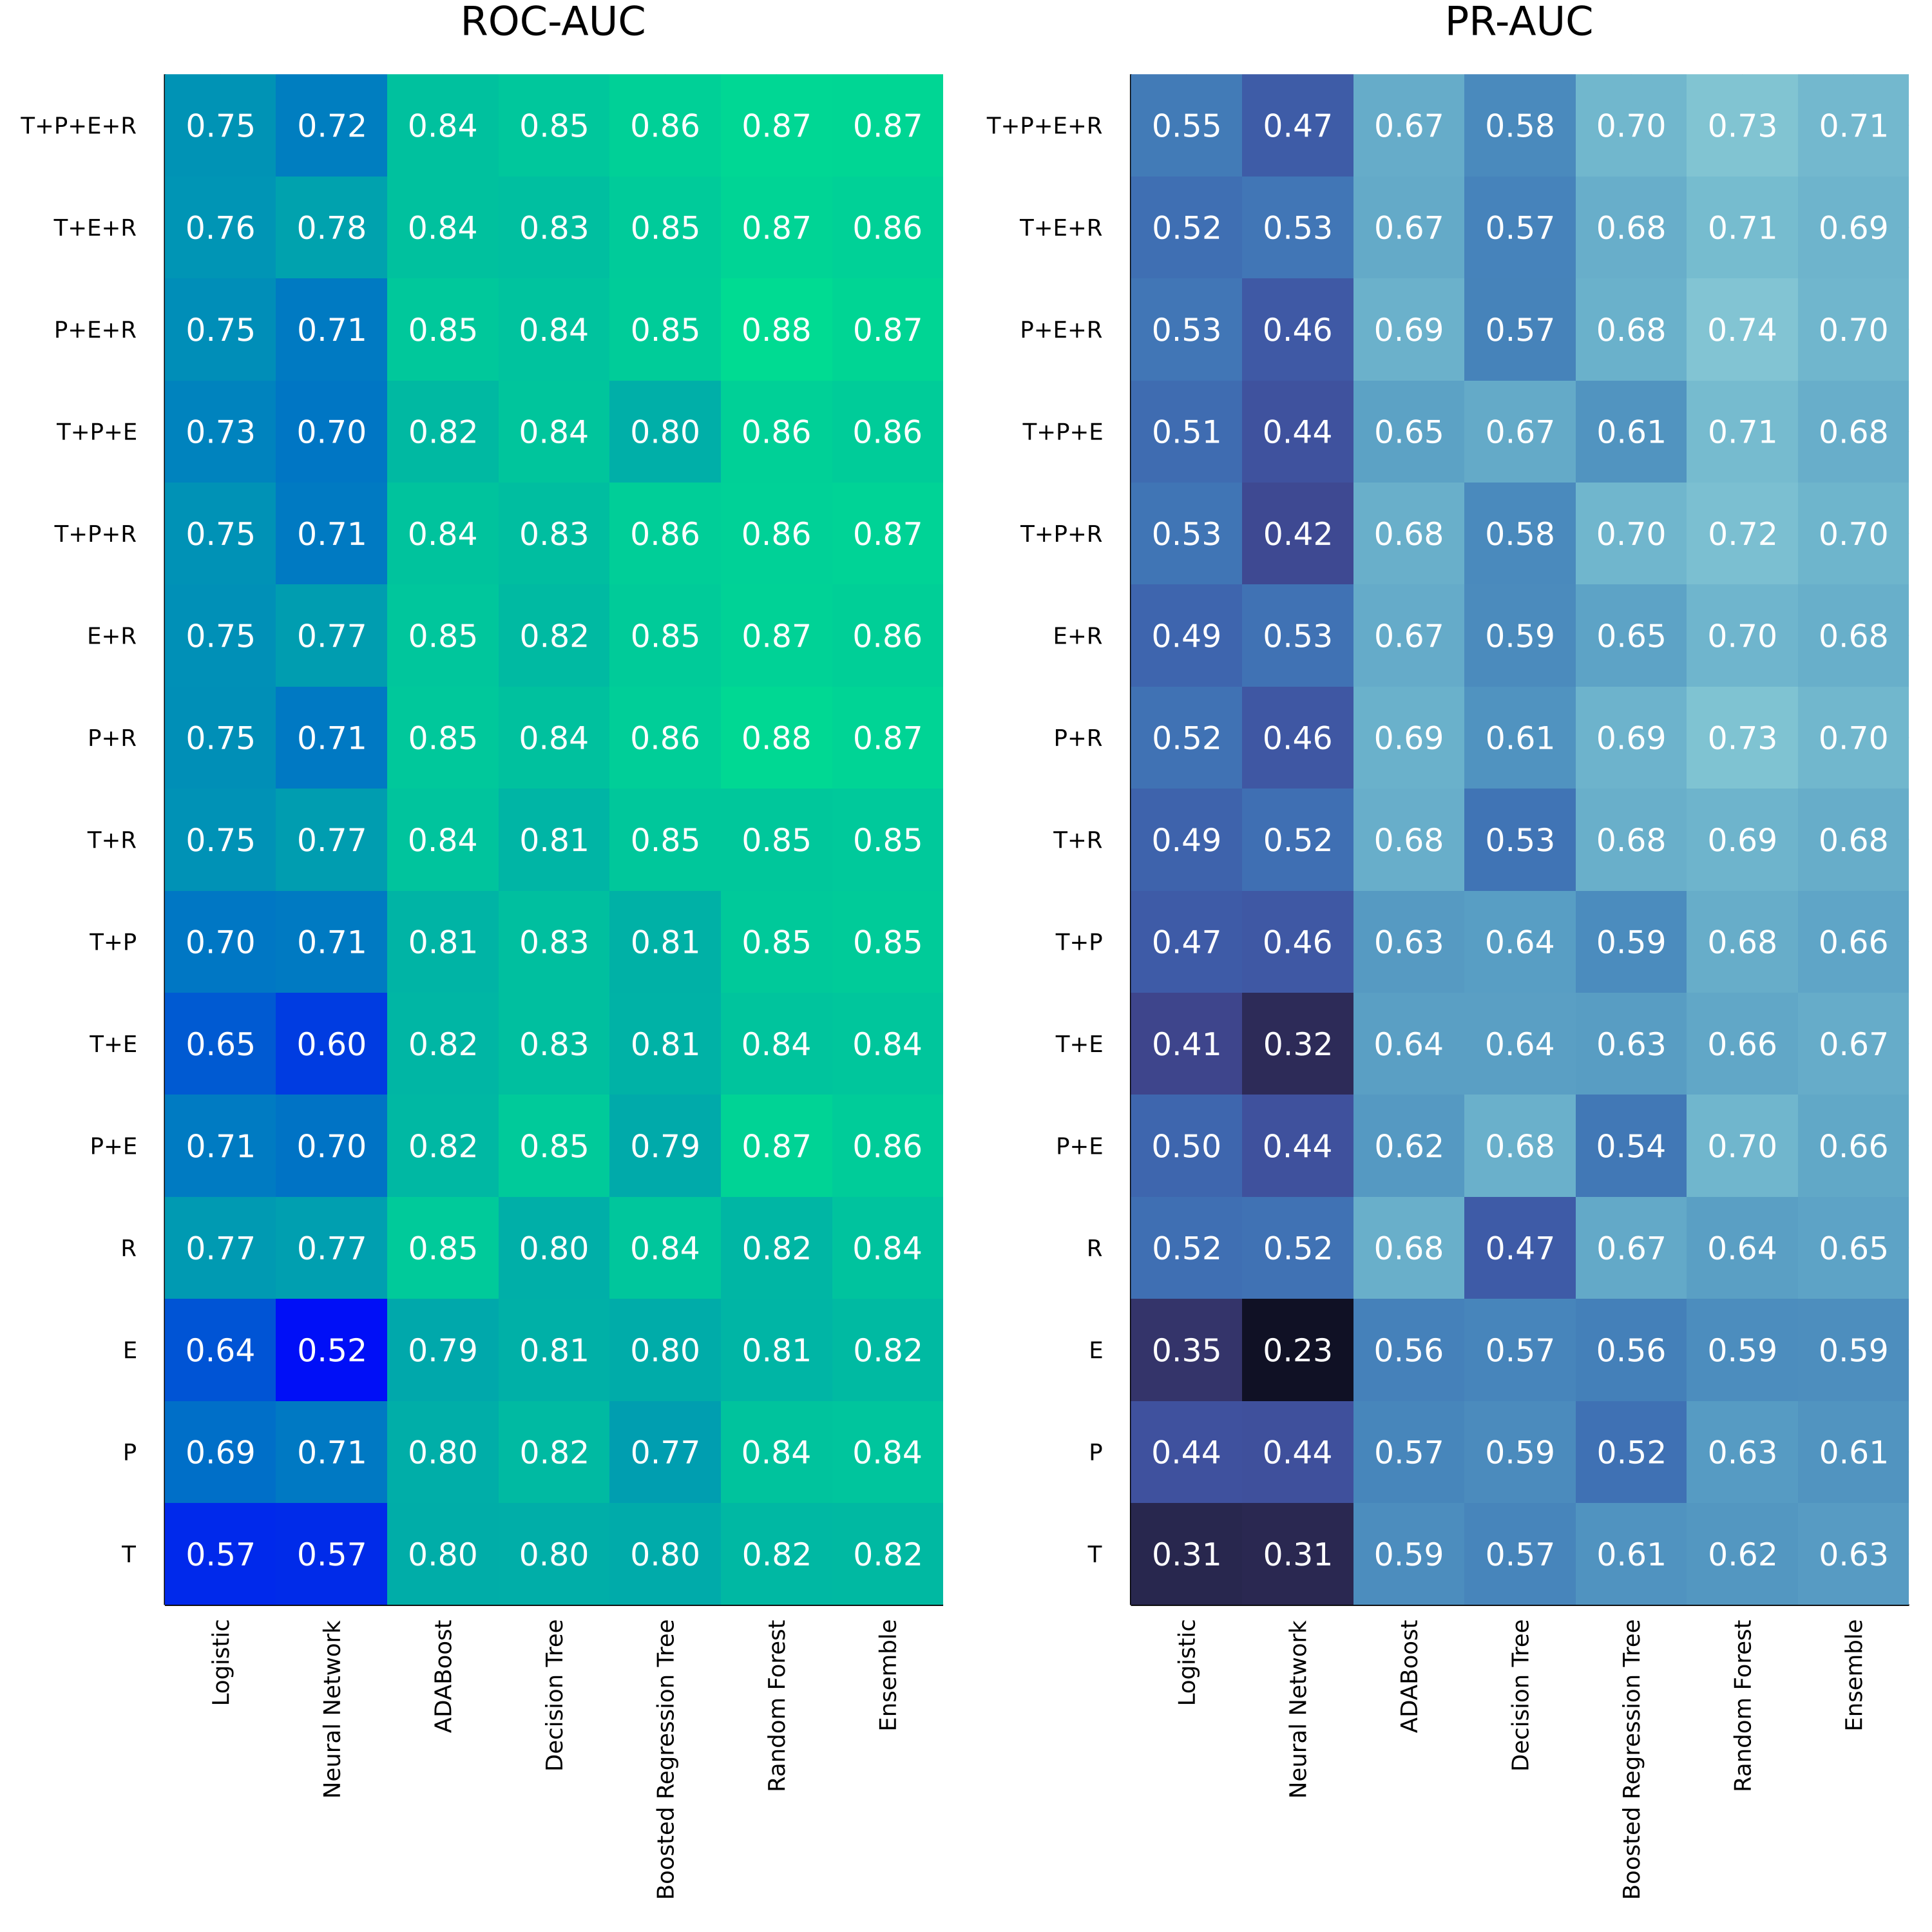
\includegraphics{./figures/PR_ROC.png}
\caption{todo}
\end{figure}

\hypertarget{spatiotemporally-explicit-networks}{%
\section{Spatiotemporally Explicit
Networks}\label{spatiotemporally-explicit-networks}}

Now that we have a metaweb\ldots..

\textbf{\emph{Figure 3: Maps over time figure and Prob(Connectance)
vs.~Month figure}}

\hypertarget{sampling-prioiritization}{%
\section{Sampling Prioiritization}\label{sampling-prioiritization}}

\textbf{\emph{Figure 4: Uncertainty and sampling priority map}}

\hypertarget{discussion}{%
\section*{Discussion}\label{discussion}}
\addcontentsline{toc}{section}{Discussion}

\hypertarget{refs}{}
\begin{CSLReferences}{1}{0}
\leavevmode\hypertarget{ref-Bascompte2007PlaMut}{}%
Bascompte, J. \& Jordano, P. (2007). Plant-Animal Mutualistic Networks:
The Architecture of Biodiversity. \emph{Annual Review of Ecology,
Evolution, and Systematics}, 38, 567--593.

\leavevmode\hypertarget{ref-Gravel2019BriElt}{}%
Gravel, D., Baiser, B., Dunne, J.A., Kopelke, J.-P., Martinez, N.D.,
Nyman, T., \emph{et al.} (2019). Bringing Elton and Grinnell together: A
quantitative framework to represent the biogeography of ecological
interaction networks. \emph{Ecography}, 42, 401--415.

\leavevmode\hypertarget{ref-Poisot2015SpeWhy}{}%
Poisot, T., Stouffer, D.B. \& Gravel, D. (2015). Beyond species: Why
ecological interaction networks vary through space and time.
\emph{Oikos}, 124, 243--251.

\end{CSLReferences}

\end{document}
